\chapter{Transport mésoscopique}

La physique mésoscopique traite des systèmes de petites tailles, habituellement de la dizaine ou de la centaine de nanomètres~(parfois moins). Le transport mésoscopique s'intéresse plus particulièrement à la façon dont les électrons vont pouvoir circuler mais aussi interagir dans ces structures nanométriques pour donner naissance à des phénomènes tels que l'effet Kondo~\cite{JKondo1} ou le blocage de Coulomb~\cite{Beenakker1991}. 

Nous allons dans ce chapitre aborder quelques notions de transport mésoscopique essentielles à la compréhension des résultats présentés dans la suite de cette thèse. Nous détaillerons dans un premier temps la structure d'un transistor à électron unique. Nous examinerons ensuite comment le courant circule au sein de cette structure et nous mettrons en évidence le phénomène de blocage de Coulomb. Nous aborderons également la notion de cotunneling, phénomène uniquement dû aux propriétés quantique du système. Enfin, nous introduirons l'effet Kondo en détaillant comment se dernier évolue en fonction des perturbation dû à l'environnement .

Quand cela sera possible, nous préciserons pour chacun de ces phénomènes les conditions nécessaires à leur observation ainsi que les variables expérimentales dont ils dépendent.
%%%%%%%%%%%%%%%%%%%%%%%%
%SECTION I
%%%%%%%%%%%%%%%%%%%%%%%%


\section{Le transistor à électron unique}
Dans le cadre de nos expériences, nous avons utilisé ce que l'on appelle un transistor à électron unique ou Single Electron Transistor~(SET). En général un tel système est composé d'un point quantique~(ou ilôt) connecté à trois terminaux que l'on nommera source, drain et grille~(en référence aux transistors à effet de champ). L'il\^ot est couplé à ces trois terminaux par trois capacitances : $C_g$ pour la grille, $C_d$ pour le drain et $C_s$ pour la source. De plus, des barrières tunnels entre le point quantique, la source et le drain permettent le passage d'électrons et sont caractérisées par les paramètres $\gamma_s$~(source/il\^ot) et $\gamma_d$~(drain/il\^ot). La source et le drain sont considérés comme des matériaux métalliques massifs dont les électrons obéissent à la statistique de Fermi-Dirac. Enfin, nous attribuons à l'il\^ot une taille caractéristique $L$. 

Ce système, les paramètres qui le caractérisent ainsi qu'un schéma électrique équivalent, sont représentés dans la Fig. \ref{description_systeme}. Nous allons maintenant détailler chacun de ces éléments.


\subsection{Les capacitances du système}
Trois capacitances couplent l'il\^ot central aux trois terminaux, et l'application d'une tension sur l'un ou plusieurs de ces terminaux va modifier l'énergie du point quantique qui s'écrit alors :

\begin{equation}
U = \frac{(C_sV_s + C_dV_d + C_gV_g)^2}{2C_{\Sigma}}
\text{   avec    } 
 C_{\Sigma} = C_g + C_s + C_g \nonumber
\end{equation}

Ces capacitances vont également induire un "co\^ut" énergétique à l'ajout d'un électron dans l'il\^ot central. Cet ajout est associé à l'énergie $E_c$, appelée énergie de charge, dont la valeur est donnée par :
\begin{eqnarray}
\frac{E_c}{2} = \frac{e^2}{2C_{\Sigma}} \nonumber
\end{eqnarray}

Si aucun électron de la source ou du drain ne possède l'énergie correspondante à $E_c$, ils ne peuvent plus circuler au sein de la structure. Le courant devient nul et l'on se retrouve en régime de blocage de Coulomb. Pour que cette situation puisse être observée, il faut que l'énergie thermique soit telle que $E_c \ll k_bT$.

En tenant compte de ces deux contributions, l'énergie d'un il\^ot contenant $N$ électrons et soumis aux tensions $V_g$, $V_d$ et $V_s$ est donnée par :
\begin{eqnarray}
U(N) = \frac{1}{2C_{\Sigma}} (-|e|N + C_sV_s + C_dV_d + C_gV_g)^2
\end{eqnarray}

On inclut parfois dans cette expression une charge $eN_0$ pour tenir compte de l'environnement électrostatique. Nous verrons, en abordant la notion de potentiel chimique, que seule la différence d'énergie entre les différents états de charge importe. Le décalage de charge introduit par ce dernier terme peut donc \^etre ignoré. \newline

\fbox{\begin{minipage}{0.9\textwidth}
\textbf{Remarque :} Dans les expériences de Microscopie à Effet Tunnel ou Scanning Tunneling Microscopie~(STM), seules les tensions de source et de drain peuvent \^etre modifiées. Cet inconvénient est compensé par la possibilité de modifier les paramètres de couplage $\gamma$~(que l'on détaillera dans la suite) en modulant la distance séparant la pointe de l'échantillon.
\end{minipage}}

\begin{figure}
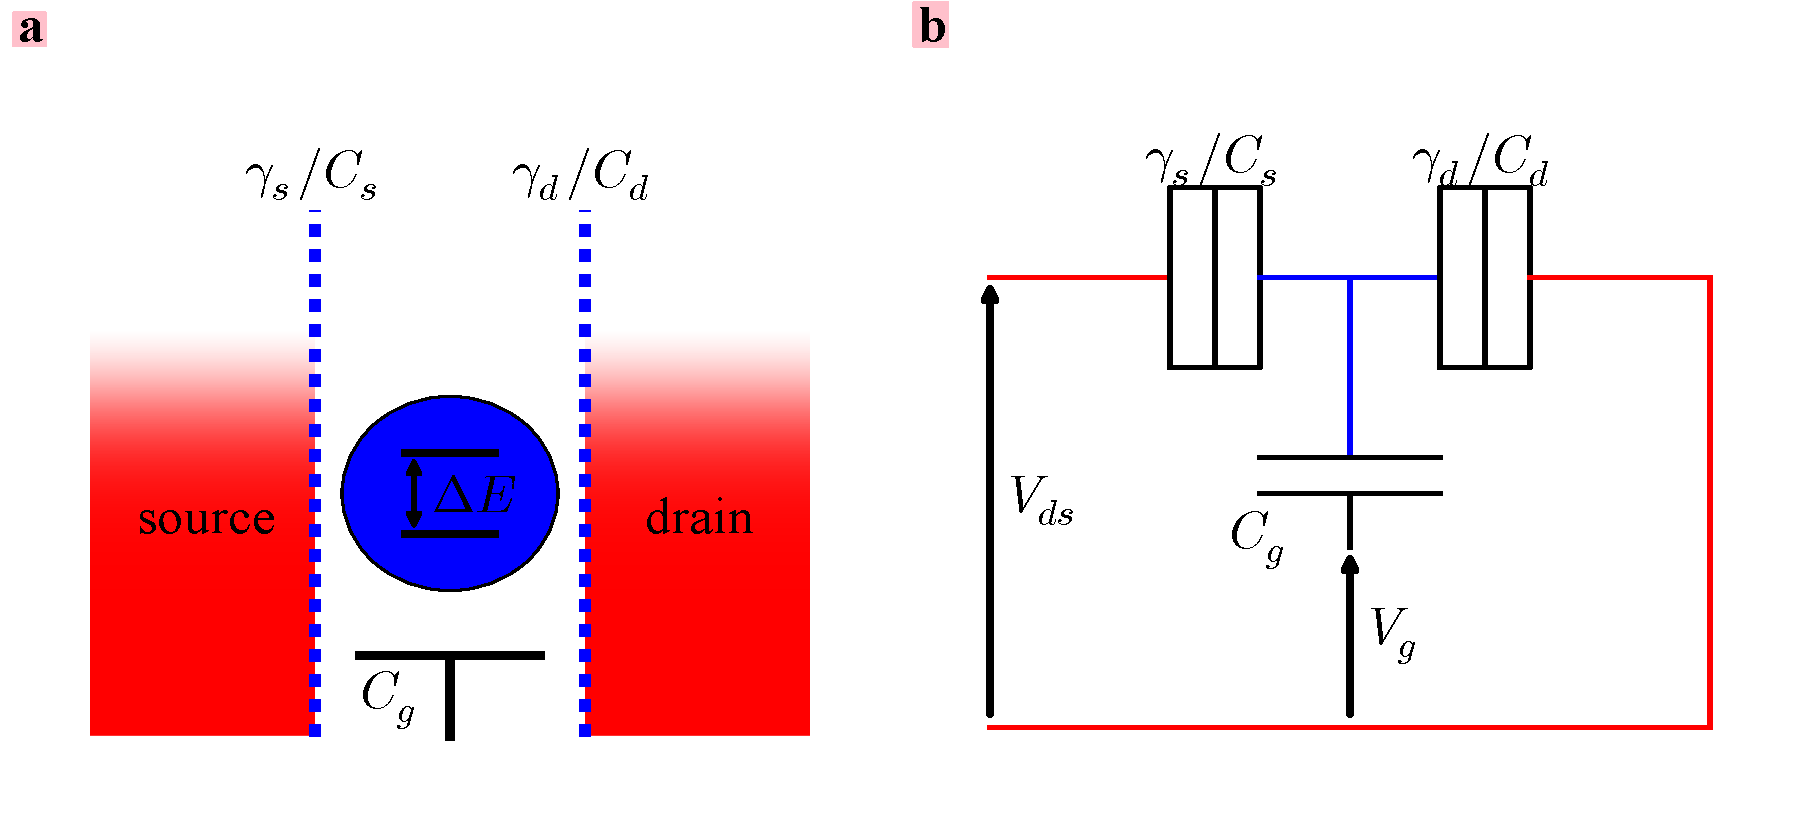
\includegraphics[scale=0.5]{Theorie/Transport/figure1/figure1.pdf} 
\caption{\textbf{a} : schémas d'un transistor à électron unique. \textbf{b} : schémas électrique équivalent.}
\label{description_systeme}
\end{figure}



\subsection{L'il\^ot}
On rencontre généralement trois types de système pouvant jouer le rôle de point quantique :
\begin{itemize}
\item \textbf{un gaz d'électron bidimensionnel~(ou 2DEG en anglais)~\cite{Gordon1}:} généralement une hétérostructre de semi-conducteur est utilisé pour obtenir un gaz d'électron bidimmensionnel proche de la surface. Par des techniques de lithographie, des électrodes sont ajoutées sur l'échantillon. En appliquant une tension sur ces grilles, le gaz d'électron peut \^etre manipulé pour former un ou plusieurs points quantiques connectés à plusieurs électrodes.
\item \textbf{un grain métallique~\cite{Deshmukh2002}:} un grain de métal~(souvent noble) de quelques nanomètres joue le rôle de point quantique. Ces grains peuvent \^etre notamment obtenus en utilisant les techniques d'évaporation ou d'électromigration.
\item \textbf{une molécule \cite{Reed1,Park1}:} les molécules susceptible de jouer ce r\^ole sont bien trop nombreuses pour toutes \^etre citées. On peut cependant donner quelques exemples célèbres : les nanotubes, les fullerènes~\cite{Park1}, les aimants moléculaires~\cite{Heersche2006} etc.. \newline
\end{itemize}

Dans le cas d'un 2DEG ou celui d'un grain métallique, du fait de la taille typique des échantillons~($\sim 100nm$ pour les premiers, $\sim 10nm$ pour les seconds), on observe une quantification des différents états du système. Le spectre énergétique de l'\^ilot peut s'exprimer en fonction de trois nombres quantiques $n_x$, $n_y$ et $n_z$ à travers la relation suivante:
\begin{eqnarray}
E_n = \frac{\pi^2 \hbar^2}{2m}(\frac{n_x^2}{L_x^2} + \frac{n_y^2}{L_y^2} + \frac{n_z^2}{L_z^2}) \nonumber
\end{eqnarray}
où $L_x$, $L_y$ et $L_z$ sont les dimensions caractéristiques de l'échantillon suivant les axes $x$,$y$ et $z$.

Il s'agit d'une expression très simplifiée car elle suppose une forme de potentiel de confinement difficile~(pour ne pas dire impossible) à obtenir en pratique (variation abrupte et hauteur de potentiel infini). Elle a le mérite en revanche de faire appara\^itre une deuxième condition nécessaire à l'observation de ce que l'on appelle habituellement le blocage de Coulomb quantique (par opposition au blocage de Coulomb classique où seul la quantification de la charge joue un rôle). En effet, pour résoudre le spectre énergétique de l'il\^ot, l'énergie thermique doit \^etre négligeable devant celle séparant deux niveaux, à savoir:

\begin{eqnarray}
\frac{\hbar^2}{2mL^2} \gg k_bT \nonumber
\end{eqnarray}

Lorsque des molécules sont utilisées, cette quantification apparaît beaucoup plus naturellement à travers la notion d'orbitales moléculaires. En effet, c'est sur ces orbitales que vont venir s'ajouter et se soustraire les électrons. On désigne souvent la dernière orbitale contenant un électron par HOMO~(Highest Occupied Molecular Orbital) et la première orbitale ne contenant aucun électron est désignée par le terme LUMO~(Lowest Unoccupied Molecular Orbital).

Il faut se garder cependant de penser qu'une molécule jouant le r\^ole de point quantique conserve les mêmes propriétés que cette m\^eme molécule isolée. Tout d'abord, les niveaux d'énergie sont fortement influencés par la présence des électrodes du fait de l'hybridisation. De plus, les électrodes peuvent induire une déformation de la molécule altérant la structure électronique de celle-ci. Ce phénomène est connu sour le nom d'effet Jhan-Teller~\cite{Jahn1937}. 

Nous montrerons par la suite que, dans le cadre de l'électronique moléculaire et plus particulièrement celui de la spintronique moléculaire, il est important de pouvoir évaluer l'influence de ces différents phénomènes.

\subsection{Les paramètre de couplage tunnel $\gamma_{s/d}$}

On peut voir ces coefficients comme définissant "l'aisance" avec laquelle les électrons peuvent passer par effet tunnel de la source ou du drain vers l'il\^ot et vice-versa. Le paramètre $\gamma$ rend également compte de l'hybridisation des niveaux d'énergie du point quantique avec ceux des électrodes. Cette hybridisation entraîne l'élargissement des niveaux d'énergie d'une largeur $\Delta E$ donnée par :
\begin{eqnarray}
\Delta E = h (\gamma_s + \gamma_d)
\label{hybridgamma}
\end{eqnarray}

Cette élargissement est appelé élargissement intrinsèque par opposition à l'élargissement induit par la température. On peut deviner ici une seconde condition nécessaire à l'apparition du phénomène de blocage de Coulomb, à savoir $\Delta E \ll E_c$. De plus, dans un régime de blocage fort, on a $\Delta E \ll k_bT$. Si cette dernière condition est remplie, on peut avoir accès aux distributions de Fermi-Dirac des électrodes et donc ,à la température du système.

La condition $\Delta E \ll E_c$ peut \^etre également reliée à la conductance du système. Celle-ci devient :
\begin{eqnarray}
E_c \tau_{RC} \ll \hbar \text{  avec  } \tau_{RC}=R_TC_{\Sigma}=C_{\Sigma}/G_T \nonumber
\end{eqnarray}
où $R_T$ est la résitance du système et $G_T$ sa conductance. Compte tenue de la définition de l'énergie de charge précédente, on en déduit :
\begin{eqnarray}
G_T << \frac{e^2}{2\hbar} \sim G_q
\end{eqnarray}
où $G_q$ est le quantum de conductance $e^2/ \hbar$. Pour observer le régime de Blocage de Coulomb, il faut que la conductance de mon SET soit largement inférieur au quantum de conductance ($\sim$ 76\,$\mu K$). On désigne cette situation par couplage faible.


\section{La notion de potentiel chimique}
La notion de potentiel chimique est, à mes yeux, une des notions les plus importantes afin de comprendre de manière simple et intuitive le phénomène de blocage de Coulomb. Un exemple de son utilisation dans la cadre du transport quantique peut \^etre trouvé dans la très belle et très pédagogique revue de Hanson \textit{et al.}~\cite{Hanson2007}. Dans cette section, nous allons tout d'abord présenter le concept de potentiel chimique. Nous exprimerons ensuite, à partir des considérations exposées dans la partie précédente, le potentiel chimique de la source, du drain et surtout de l'\^ilot central.

\subsection{Définition}

On recontre souvent le potentiel chimique en thermodynamique lorsqu'on s'intéresse aux systèmes ouverts échangeant des particules~(cf. ensemble Grand Canonique). Cette grandeur défini la variation d'énergie d'un système d\^u à la modification du nombre de particules qui le composent. On le trouve parfois défini comme suit :
\begin{eqnarray}
\mu = \frac{\partial U}{\partial N} \nonumber
\end{eqnarray}
$U$ étant l'énergie du système et $N$ le nombre de particules. Dans la suite, nous allons plut\^ot adopter la notation de \cite{Hanson2007} et prendre la définition suivante :
\begin{eqnarray}
\mu(N) = U(N) - U(N-1)
\label{potchimeq}
\end{eqnarray}
où $\mu(N)$ est le potentiel chimique de l'état de charge $N$, $U(N)$ et $U(N-1)$ étant respectivement l'énergie du système avec $N$ et $N-1$ particules.


\subsection{Les potentiels chimiques de la source et du drain.}
L'expression du potentiel chimique de la source et du drain est directement donnée par $\mu_i = e V_i$ ou $i=source/drain$. Il s'agit du niveau de Fermi des électrons dans la source et le drain (à ne pas confondre avec l'énergie de Fermi). La probabilité, dans un métal de niveau de Fermi $\mu_F$, de trouver un électron de potentiel chimique $\mu$ est donnée par la distribution de Fermi:
\begin{eqnarray}
p(\mu) = \frac{1}{1 + \exp{(\frac{\mu - \mu_F}{k_bT})}} \nonumber
\end{eqnarray}
où $k_b$ est la constante de Boltzmann et $T$ la température du système. On obtient donc en fonction des tensions source et drain:
\begin{eqnarray}
p_i(\mu) = \frac{1}{1 + \exp{(\frac{\mu - eV_i}{k_bT})}}
\end{eqnarray}
Cette notion est essentielle dans la détermination du courant qui traverse notre structure.

\begin{figure}
\centering 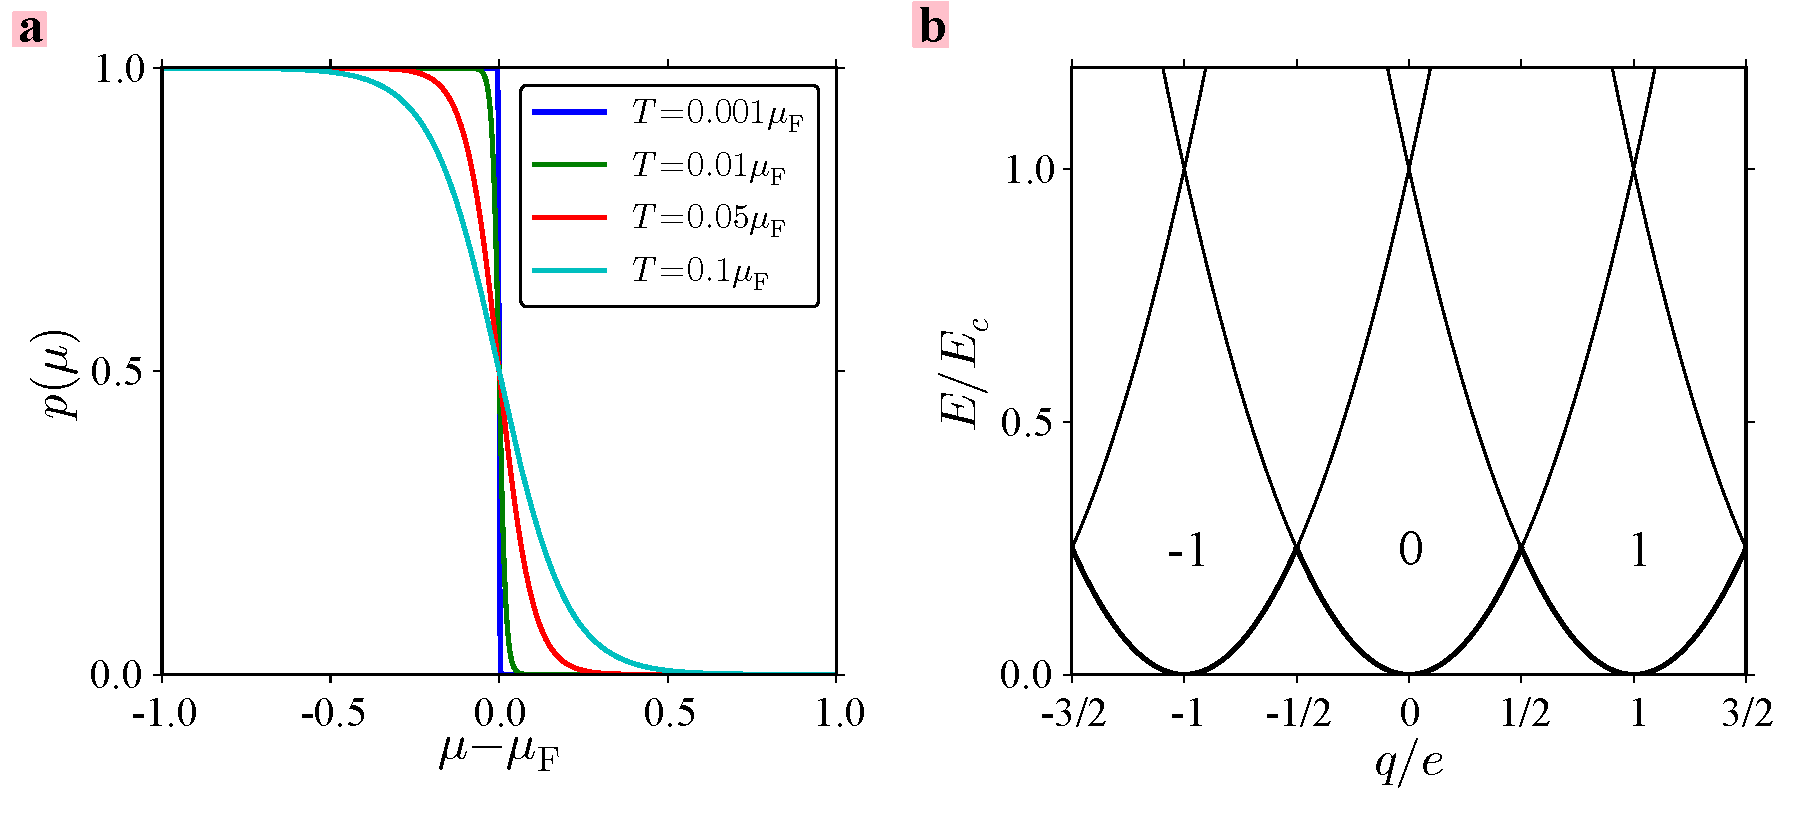
\includegraphics[scale=0.5]{Theorie/Transport/figure2/figure2.pdf} 
\caption{ \textbf{a} : probabilité d'avoir un électron de potentiel chimique $\mu$ sachant que le potentiel chimique du métal est $\mu_{\rm{F}}$ pour différent températures. \textbf{b} : évolution de l'énergie des états de charges $-1$, $0$ et $1$ en fonction de $q = -C_gV_g$. Pour des valeurs demi-entières de $q/e$, deux états de charge se retrouvent dégénérés. On parle de point de dégénérescence~(inspiré de \cite{NazaBook}).}
\label{distrib_fermi}
\end{figure}



\subsection{Le potentiel chimique de l'il\^ot}
Lorsque l'on analyse les résultats d'une expérience, toute la difficulté réside dans la détermination du potentiel chimique de l'\^ilot. Dans la partie précédente nous avons déjà fait le bilan des différentes énergies en jeu dans le système. A savoir, nous devons prendre en compte l'énergie électrostatique, l'énergie d'interaction électron-électron ainsi que la discrétisation des niveaux d'énergie dans l'il\^ot. Tout ceci donne :
\begin{eqnarray}
U(N) = \underbrace{\frac{1}{2C_{\Sigma}} (-|e|N + C_sV_s + C_dV_d + C_gV_g)^2}_{\text{couplage électrostatique et énergie de charge}}
+ 
\underbrace{\sum_{n=1}^{N} E_n}_{\substack{\text{énergie liée aux} \\\text{aux états discrets}}}
\end{eqnarray}

On peut également tenir compte de l'application d'un champ magnétique en attribuant à chaque niveau discret, une dépendance en champ magnétique :
\begin{eqnarray}
\sum_{n=1}^N E_n = \sum_{n=1}^N E_n(B) \nonumber
\end{eqnarray}
On se retrouve, d'après la définition du potentiel chimique de l'Eq.\ref{potchimeq}, avec une expression relativement simple :
\begin{eqnarray}
\mu(N) = (N-\frac{1}{2})\frac{e^2}{C_{\Sigma}}
+ 
\frac{e}{C_{\Sigma}}(C_gV_g + C_sV_s + C_dV_d)
+
E_N(B)
\end{eqnarray}

En introduisant l'énergie de charge $E_c$ introduite précédemment, nous pouvons réécrire la relation sous la forme:

\begin{eqnarray}
\mu(N) = (N-\frac{1}{2})E_c
- 
\frac{E_c}{|e|}(C_gV_g + C_sV_s + C_dV_d)
+
E_N(B)
\label{pot_chim}
\end{eqnarray}

L'énergie $E_c$ est donc l'énergie d\^u à la répulsion Coulombienne qui sépare deux potentiels chimiques d'état de charge consécutifs.


\section{Le blocage de Coulomb}
Pour rendre l'exposé qui va suivre plus clair, nous allons le décomposer en trois parties. Dans la première partie, nous analyserons les conditions à remplir pour qu'un électron du drain puisse aller dans l'il\^ot. Dans la deuxième, nous ferons de m\^eme pour la source. Enfin, nous exploiterons les résultats obtenus pour en déduire les conditions nécessaires à la circulation d'un courant. Afin d'adapter les solutions trouvées aux conditions expérimentales, on posera $V_s = 0$ car dans la grande majorité des dispositifs, une des électrodes est directement connectée à la masse. Ce qui donnera $V_d=V_{ds}$, $V_{ds}$ étant la tension appliquée à l'échantillon.

\subsection{Charge de l'\^ilot par le drain}
Supposons l'\^ilot dans l'état de charge $N-1$, pour passer à l'état de charge $N$, il faut qu'il y ait au moins un électron dans le drain dont le potentiel chimique soit égal à $\mu(N)$. Il nous suffit d'observer la courbe de la Fig. \ref{distrib_fermi}.a pour comprendre que cela suppose :
\begin{eqnarray}
p(\mu) > 0 \Longrightarrow  -|e|V_{ds} \geq \mu(N) \nonumber
\end{eqnarray}

Ce qui conduit à la relation suivante :
\begin{eqnarray}
-|e|V_{ds} \geq (N-\frac{1}{2})\frac{e^2}{C_{\Sigma}}
-
\frac{|e|}{C_{\Sigma}}(C_gV_g + C_sV_s + C_dV_d)
+
E_N(B) \nonumber
\end{eqnarray}

En tenant compte des conditions $V_s= 0$ et $V_{ds} = V_d$ évoquées plus haut, cette relation peut se réécrire:
\begin{eqnarray}
V_{ds} \leq \frac{1}{C_g + C_s} \left\lbrace C_gV_g - \frac{C_{\Sigma}}{|e|}\left(E_N(B) + (N-\frac{1}{2})E_c \right) \right\rbrace 
\end{eqnarray}

La zone de transition entre charge et décharge de l'\^ilot dans le plan ($V_g$,$V_{ds}$) est délimité par une droite dont la pente $\dfrac{C_g}{C_g + C_s}$ dépend des différentes valeurs de capacitances du système.


\begin{figure}
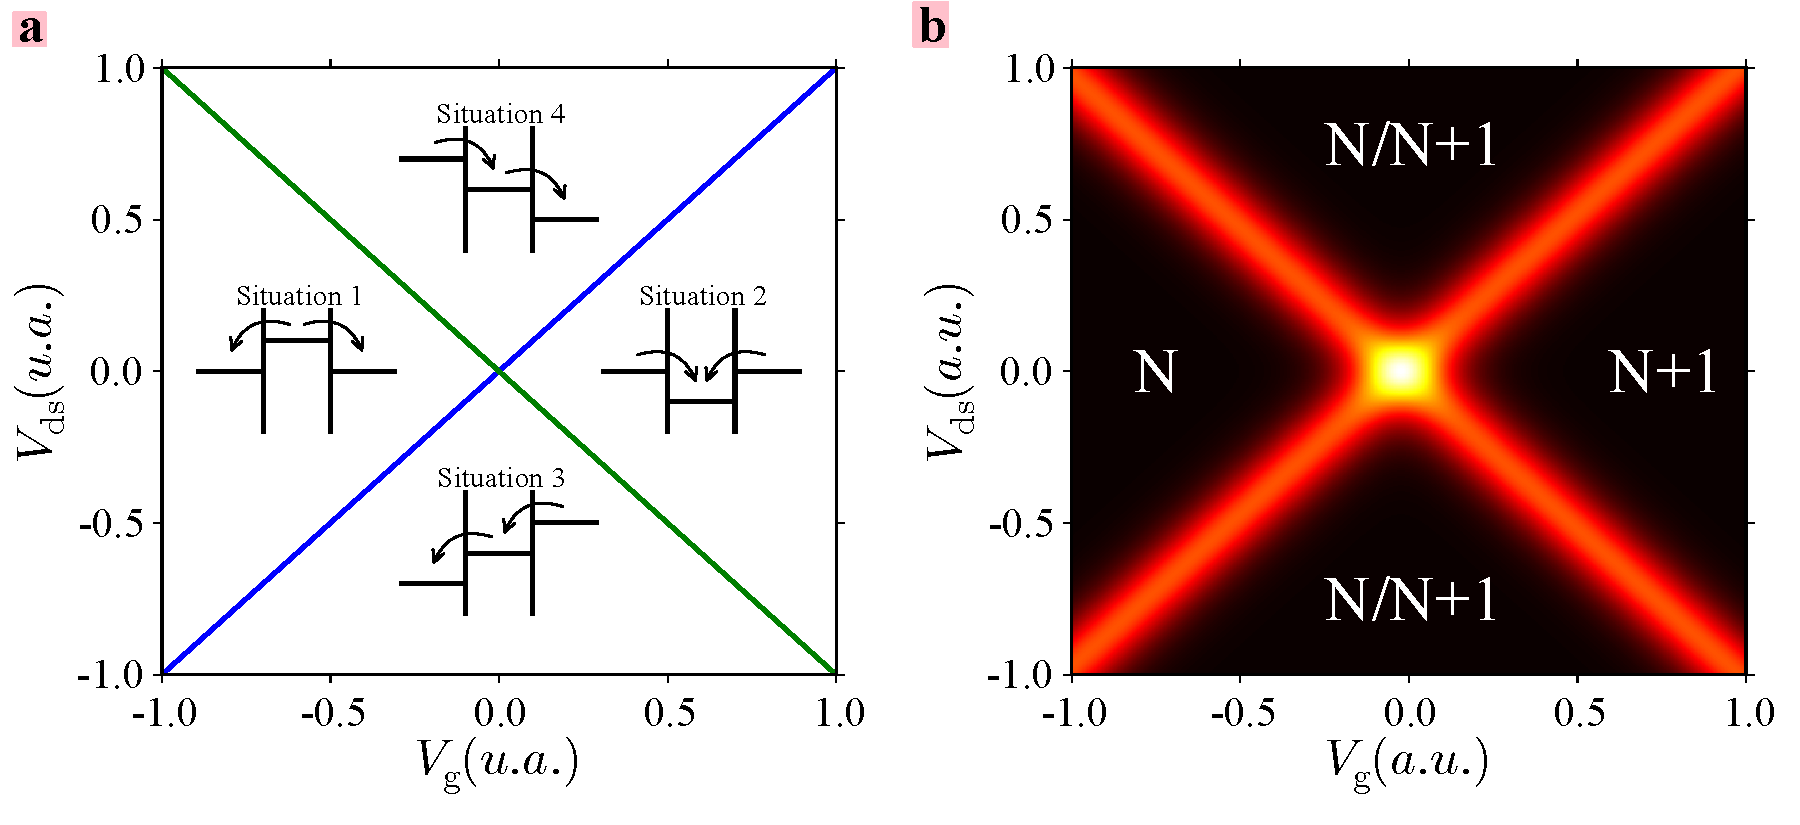
\includegraphics[scale=0.5]{Theorie/Transport/figure3/figure3.pdf} 
\caption{\textbf{a} : représentation de la charge et de la décharge de l'il\^ot dans le plan ($V_g$,$V_{ds}$). Le régime de blocage de Coulomb est représenté par les situations 1 et 2. Un courant est mesuré dans les situations 3 et 4. \textbf{b} : m\^eme digramme obtenue en mesurant la conductance différentielle $dI/dV$ en fonction des tension $V_g$ et $V_{ds}$. La valeur de la conductance différentielle est basse pour les zones sombres et élevée pour les zones claires.}
\label{charge_discharge}
\end{figure}



\subsection{Charge de l'il\^ot par la source}
Un raisonnement similaire au précédent conduit à la relation suivante :

\begin{eqnarray}
V_{ds} \geq -\frac{1}{C_d} \left\lbrace C_gV_g + \frac{C_{\Sigma}}{|e|}\left( E_N(B) + (N-\frac{1}{2})E_c \right) \right\rbrace
\end{eqnarray}


La pente $-\dfrac{C_g}{C_d}$ correspond alors à la charge ou la décharge de l'il\^ot par la source (cf Fig.\ref{charge_discharge})

Nous pouvons également déduire de ce qui précède une deuxième relation importante. Deux points de dégénérescence sont séparés par une tension de grille $\Delta V_g$ que l'on peut relier aux paramètres du système par la formule suivante:
\begin{eqnarray}
\frac{C_g}{C_{\Sigma}} |e| \Delta V_g = E_c + \Delta E
\end{eqnarray}
où $\Delta E = E_N(B) - E_{N-1}(B)$ est l'écart entre deux niveaux d'énergie du spectre discret.



\subsection{Condition de circulation du courant}

Si l'on reprend les deux paragraphes précédents, on peut envisager les quatre situations représenté sur la Fig. \ref{charge_discharge}. Dans les situations un et deux, l'état de charge de l'il\^ot est bien défini et on se trouve dans le régime de blocage de Coulomb. Dans la situation 3, les électrons circulent du drain vers la source. Un courant négatif est mesuré. Dans la situation 4 les électrons circulent de la source vers le drain. Un courant positif est donc mesuré.

Souvent, les mesures ne se font non pas en courant, mais en conductance différentielle $dI/dV$. Cetre mesure est préférée à celle en courant DC car elle peut \^etre faite par un technique de détection synchrone~(lock-in en anglais) qui à l'avantage de fournir des mesures plus "propres" et donc plus facilement exploitables. Une simulation d'une telle mesure obtenue par la méthode des équations pilotes est présenté dans la  Fig.\ref{charge_discharge}.b. Les différentes zones décrites précédemment sont séparées par de grandes variations dans la conductance différentielle mesurée.\newline


\fbox{\begin{minipage}{0.90\textwidth}
\textbf{Remarque :} dans le cas d'une tension source-drain nulle, la condition de circulation de courant impose $\mu(N)=0$ soit $U(N)=U(N-1)$. Les deux états de charge sont dégénérés et on parle alors de point de dégénérescence. Un représentation de l'énergie $U(N)$ pour différents états de charge est représenté dans la Fig.\ref{distrib_fermi}.b.
\end{minipage}}



\section{Etats excités et transport}

Dans de nombreux cas, une transition d'un état de charge à l'autre ne peut pas être associée à un unique potentiel chimique du fait de la présence d'états excités pour l'un ou les deux états de charges. Il faut donc prendre en compte toutes les transitions afin de déterminer correctement la signature du transport. Pour illustrer ceci, nous allons prendre un exemple simple dans lequel une boite quantique oscille entre les états de charges $N=0/1$. De plus, nous tiendrons compte du spin de l'électron. 

On va distinguer deux transitions : la transition d'un état de charge $N=0$ à un état de charge $N=1$ avec un état de spin up~($0\rightarrow +$) sera associée au potentiel chimique $\mu_{+}$; la transition d'un état de charge $N=0$ à un état de charge $N=1$ avec un état de spin down~($0\rightarrow -$) sera quant à elle associée au potentiel chimique $\mu_{-}$. Sans champ magnétique appliqué, le potentiel chimique $\mu_{+}$ possède la m\^eme énergie que le potentiel chimique  $\mu_{-}$.

Si l'on applique un champ magnétique au système, du fait de l'effet Zeeman, la dégénérescence des deux états de spin est levée (cf Fig. \ref{charge_discharge}.b). Les deux potentiels chimiques $\mu_{-}$ et $\mu_{+}$ n'ont plus la même énergie. Le premier correspond désormais à la transition entre deux états fondamentaux~($EF(0)\rightarrow EF(1)$). Le second correspond à la transition de l'état fondamental de $N=0$ à l'état excité de $N=1$~($EF(0)\rightarrow EE(1)$).

On peut construire deux jeux de diamants de Coulomb, l'un correspondant à $\mu_{-}$ et l'autre à $\mu_{+}$~(cf Fig. \ref{charge_discharge}.a en bleu et rouge respectivement). Cependant, dans les zones de blocage associé au diamant de la transition $EF(0)\rightarrow EF(1)$ (représenté ici par le potentiel chimique $\mu_{-}$) , aucun courant ne peut circuler (zone grisée dans la Fig.\ref{charge_discharge}.a). Les bords de diamant situés dans cette zone doivent apparaître en pointillé car ils ne correspondent pas réellement à une modification du courant.

De part cette construction, on constate que l'intersection entre les bords de diamants de la transition $EF(0)\rightarrow EE(1)$ et ceux de la transition $EF(0)\rightarrow EF(1)$ donne une lecture directe de l'effet Zeeman (cf Fig. \ref{charge_discharge}.a). On peut, par une mesure de transport, faire la spectroscopie du point quantique en fonction du champ magnétique.

 Cependant, dans la plupart des cas, les états N/N+1 possèdent tous deux des états fondamentaux et des états excités et l'analyse de la signature du système en transport devient plus difficile. Ces différentes configurations sont notamment traitées par Hanson \textit{et al.}, et un exemple peut \^etre trouvé dans l'analyse du $N@C_{60}$ proposée dans \cite{Grose2008}.

\begin{figure}
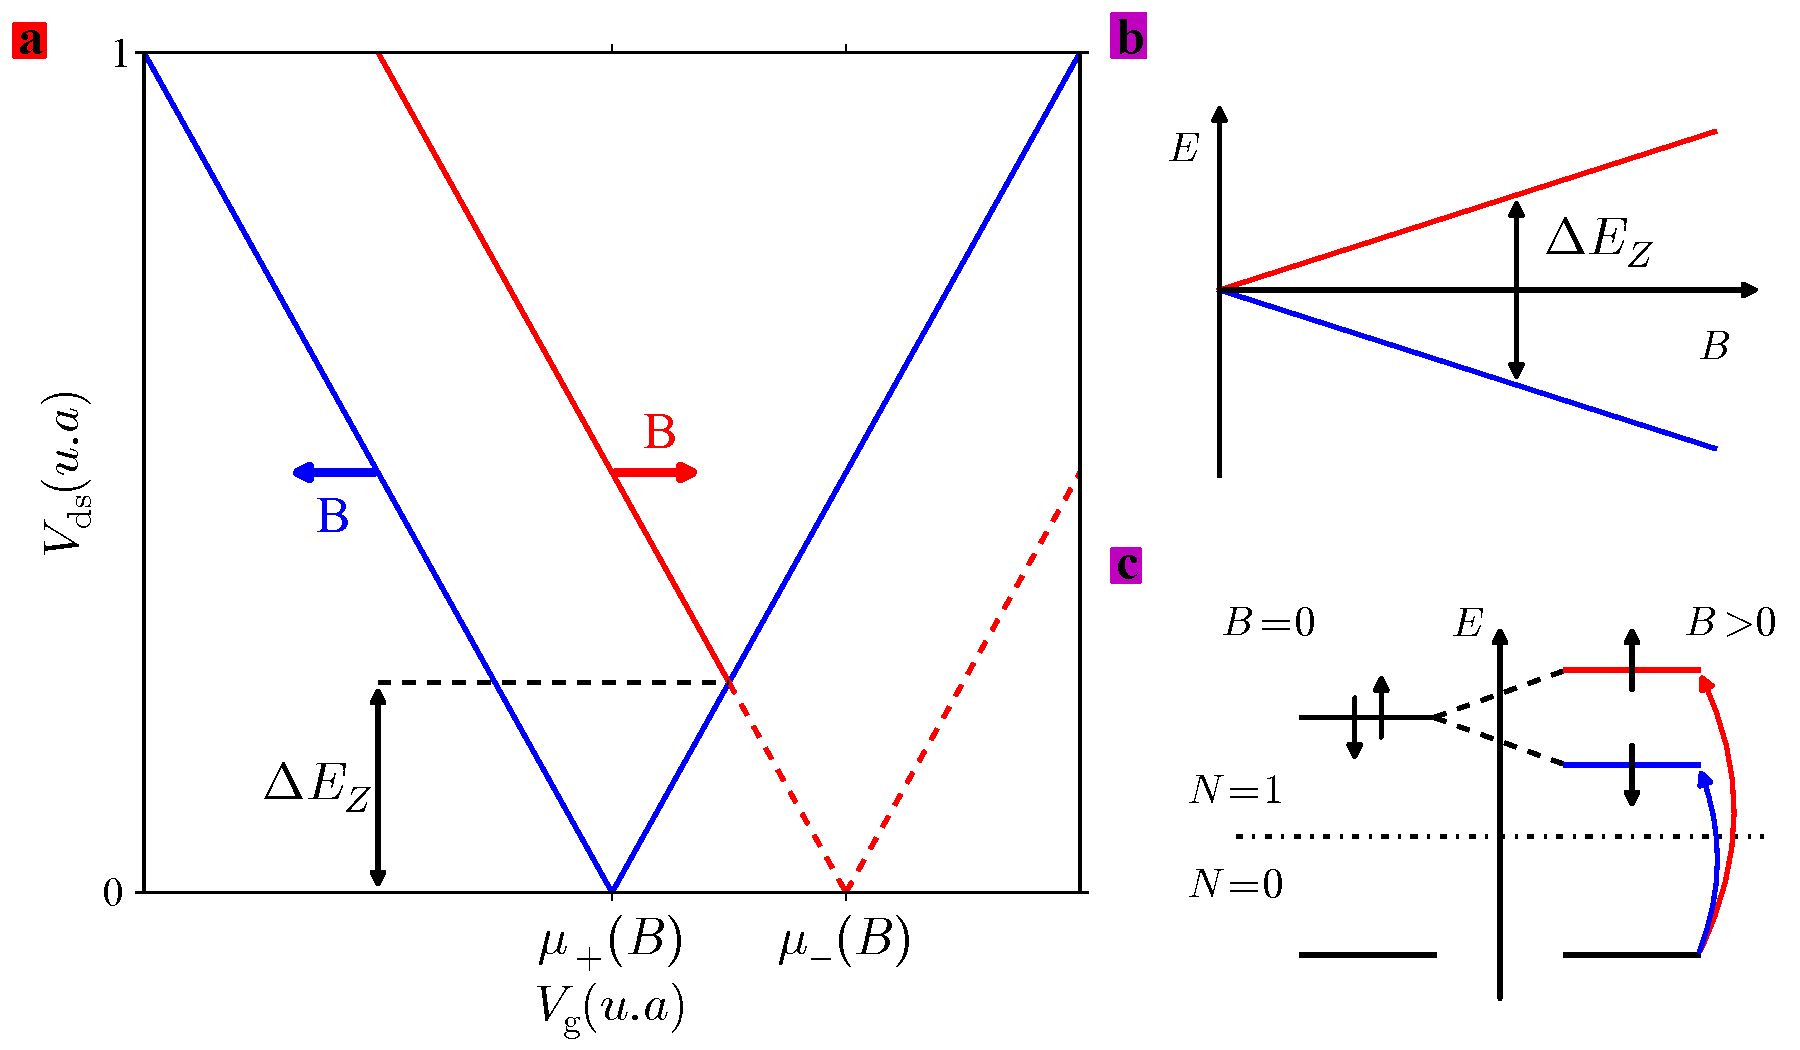
\includegraphics[scale=0.5]{Theorie/Transport/figure4/figure4.pdf} 
\caption{ \textbf{a} : diagramme de stabilité tenant compte des états fondamentaux et excités. L'influence du champ magnétique est directement mesurable au niveau des croisement des bords de diamant qui nous donnent une lecture directe de l'énergie de Zeeman $E_z$. \textbf{b} : diagramme Zeeman de l'état de charge N=1. L'application d'un champ magnétique lève la dégénérescence entre les deux spins de l'énergie Zeeman $E_z$. \textbf{c} : potentiel chimique correspondant à la transition 0/1. L'influence du champ magnétique vient levé la dégénérescence des deux états de spin et donc des deux potentiels chimiques correspondants.}
\label{etat_excite}
\end{figure}

\section{Cotunneling}
Nous avons vu jusqu'à maintenant que dans les zones de blocage de Coulomb, l'état de charge du système est fixe du fait de l'énergie de charge. En effet, l'ajout d'un électron supplémentaire aurait un "co\^ut" énergétique trop grand pour le système. Cependant, de part les inégalités d'Heinsenberg, un système peut outrepasser cette limitation pendant un temps très court. L'ordre de grandeur de ce temps dépend de l'énergie nécessaire et est donné par la relation :
\begin{eqnarray}
\tau \simeq \frac{\hbar}{E_c} \nonumber
\end{eqnarray}


\begin{figure}
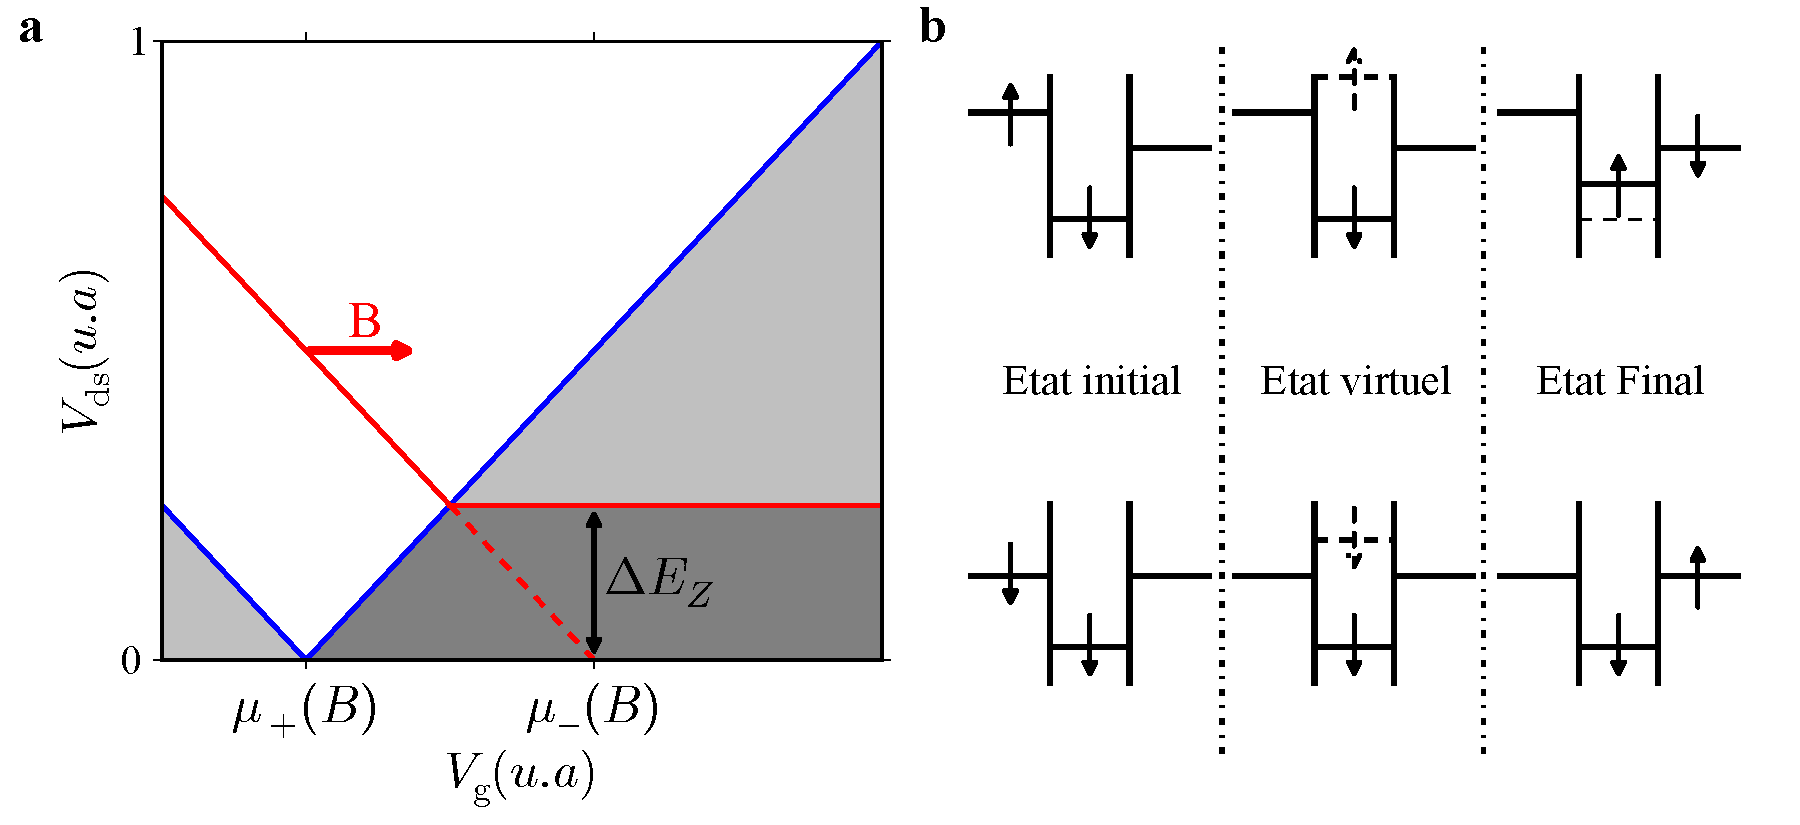
\includegraphics[scale=0.5]{Theorie/Transport/figure5/figure5.pdf} 
\caption{\textbf{a} : représentation du cotunneling dans le plan ($V_g$,$V_{ds}$). Ce dernier est responsable de la présence de courant dans les zones de blocage. Ce courant peut varier au sein de cette zone comme le montre les deux niveaux de gris. \textbf{b} : représentation des trois temps du cotunneling inélastique. L'état final de l'il\^ot est de plus haute énergie que l'état initial. \textbf{c} :  représentation des trois temps du contunneling élastique. L'énergie de l'il\^ot entre l'état initial et l'état final est identique.}
\label{cotun}
\end{figure}


Une façon de voir le phénomène est de dire que pendant le temps $\tau$ un électron est entré dans le point quantique pendant qu'un autre en est sorti, d'où l'appellation de "cotunneling". Si un m\^eme état de charge possède plusieurs états~(fondamentaux et excités), on peut imaginer deux situations. Dans le premier cas, l'électron entrant vient occuper un état de m\^eme énergie que celui de l'électron sortant et dans ce cas on parle de cotunneling élastique. Si l'électron entrant occupe un état d'énergie plus élevée que l'électron sortant, alors on parle de cotunneling inélastique. Dans le deuxième cas, cette différence en énergie que l'on notera $\Delta E_{cot}$ dans la suite doit être fournie au système. Ce rôle est assuré par la tension $V_{\rm{ds}}$ et pour qu'un processus inélastique ait lieu, il faut donc que :
\begin{eqnarray}
|e|V_{\rm{ds}} \geq \Delta E_{cot}
\end{eqnarray}

Dans le cas du cotunneling élastique cette condition est toujours remplie. C'est ce phénomène qui donne le fond de conductance. Dans la zone de blocage de Coulomb, on va donc observer des zones avec des valeurs de conductance différentielle différentes~(cf nuance de gris Fig.\ref{charge_discharge}.a). Dans le cas présenté ici, la limite entre les deux zones permet une lecture directe de l'effet Zeeman $\Delta E_z$. Encore une fois, il s'agit ici d'un cas simple avec un unique état excité. Un étude plus complexe peut \^etre trouvés dans \cite{DeFranceschi2001} ains que dans l'article en fin de thèse concernant la molécule d'endofullrène.\newline

\fbox{\begin{minipage}{0.9\textwidth}
\textbf{Remarque :} Je voudrais ici insister sur la différence entre la spectroscopie en tunneling et celle en cotunneling. La première s'intéresse aux transitions entre deux états d'énergie relatif à deux états de charges différents. Il faut donc "deconvoluer" le signal pour pouvoir analyser le spectre des deux états de charge. Dans le cas du cotunneling, on peut accéder directement aux spectres d'un état de charge donné. Les règles de sélection des transitions sont également différentes. Dans le cas du tunneling, on doit avoir $\Delta m = \pm 1/2$. Pour le cotunneling, cette règle de sélection devient $\Delta m = 0 \text{ ou } \pm 1$. Il peut arriver que des états inaccessibles par une spectroscopie en régime de tunneling soient en revanche accessibles par une mesure en régime de cotunneling. Une comparaison des deux méthodes peut \^etre trouvée dans l'article en fin de thèse ainsi que dans la thèse de Nicolas Roch.
\end{minipage}}


\section{Effet Kondo}

Tout comme le blocage de Coulomb, l'effet Kondo a d'abord été mesuré sur des échantillons macroscopiques consistant en un metal massif contenant des impuretés magnétiques. En mesurant la conductance de ces échantillons, les expériences avaient montré une anomalie. Celle-ci qui aurait d\^u diminuer durant le refroidissement ne suivait cette tendance que jusqu'à une certaine température pour augmenter à nouveau. Ce problème est resté insoluble pendant quelques années jusqu'au modèle proposé par Jung Kondo en 1964~\cite{JKondo1}. Ce modèle est relativement simple à concevoir mais en revanche très difficile à résoudre car faisant appel à la physique à $N$ corps. Dans ce modèle, les électrons de conduction viennent se coupler de façon antiférromagnétique aux impuretés du métal de telle sorte que le moment magnétique total devient nul. Chaque impureté agit donc comme un centre de diffusion très actif diminuant d'autant la conductance du système. La physique à $N$ corps apparait au travers des électrons de conduction. En effet, l'impureté magnétique interagit avec un grand nombre d'électrons que l'on désigne par le terme de "nuage Kondo". Le seul problème du modèle à l'époque, c'est qu'il prevoit une divergence de la conductance quand la température tend vers zéro. Il faudra attendre encore quelques années avec la théorie de renormalisation~(NRG en anglais) proposée par Wilson~\cite{Wilson1975}, pour résoudre complètement le problème.

Récemment la physique mésoscopique a permis de mettre à la disposition des théoriciens des modèles plus simples à résoudre dans lesquels le nombre d'impuretés magnétiques pouvait être réduit à l'unité et le couplage aux électrons pouvait être contrôlé de manière précise. Les 2DEGs, par exemple, permettent un contrôle quasi-parfait de ces différents paramètres. La littérature est riche en articles et revues de toutes sortes couvrant de nombreux aspects de l'effet Kondo. Notre groupe à notablement contribuer à l'investigation de cette physique au travers notamment de l'étude de la transition de phase quantique~\cite{Roch2008} et de l'effet Kondo sous écranté~\cite{Roch2009}. Cependant, je ne traiterai pas en détail de ces effets.

\begin{figure}
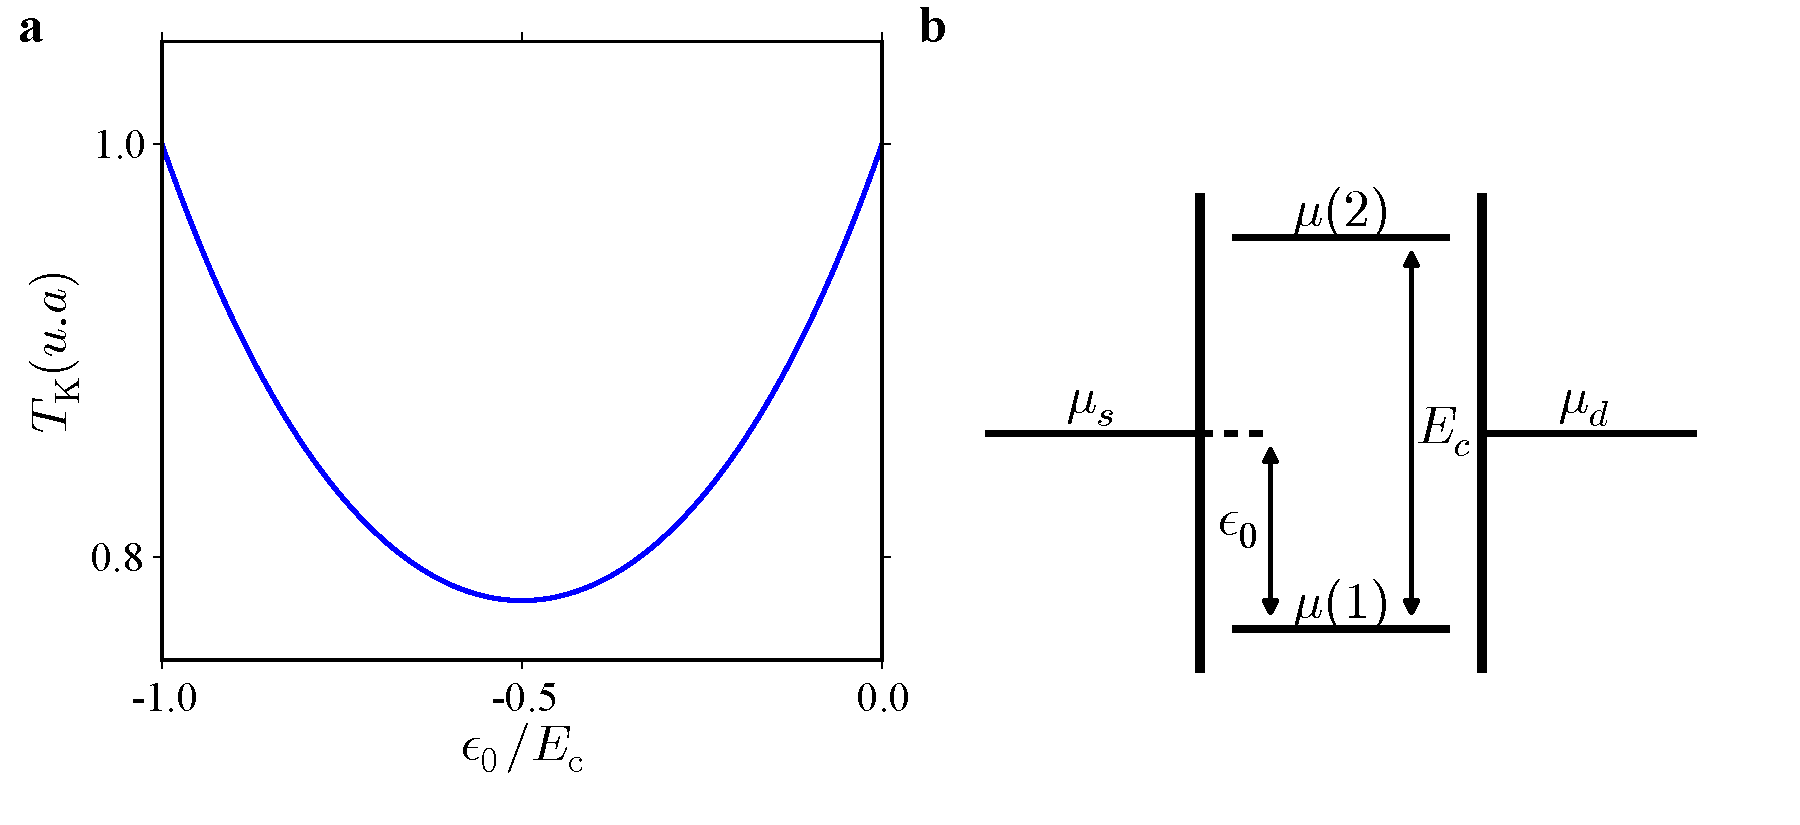
\includegraphics[scale=0.5]{Theorie/Transport/figure6/figure6.pdf} 
\caption{\textbf{a} : évolution de la température Kondo en fonction du paramètre $\epsilon_0$. Celle-ci est minimale pour une valeur $\epsilon_0=-0.5$, ce qui correspond au centre d'un diamant de Coulomb. Elle est maximale pour $\epsilon_0=0$ ou $-1$, c'est à dire au niveau des points de dégénérescence. \textbf{b} : représentation schématique des différents paramètres du phénomène Kondo.}
\label{Kondo_param}
\end{figure}


Je voudrais en revanche dresser quelques généralités de l'effet Kondo dans les transistors moléculaires. Comme j'ai expliqué précédemment, l'effet Kondo~(de spin) réside dans le couplage entre une impureté magnétique et les électrons de conduction. Dans notre système, cette impureté peut être jouée par un niveau ne contenant qu'un seul électron non apparié. Il s'agit donc d'une impureté de spin $1/2$. Cette impureté est couplée aux électrons de la source et du drain. Le couplage anti-ferromagnétique n'est effectif qu'en dessous d'une température caractéristique nommée température Kondo et noté $T_K$ dans la suite. Cette température $T_K$ dépend principalement de trois paramètres : l'énergie de charge $E_c$, le couplage aux électrodes $\gamma$ et la différence en énergie entre le potentiel chimique du point quantique et le niveau de Fermi des électrodes. Ces trois paramètres sont représentés sur la Fig.\ref{Kondo_param}.b et sont liés par la relation suivante:
\begin{eqnarray}
T_K \sim \frac{\sqrt{\gamma E_c}}{2} \exp(\frac{\pi \epsilon_0(\epsilon_0 + E_c)}{2\gamma E_c})
\end{eqnarray}

Première constatation, plus l'énergie de charge $E_c$ est grande, plus la température Kondo sera élevée. C'est ici que réside un des avantages des transistors moléculaires comparativement aux 2DEGs. Les énergies de charge sont en général beaucoup plus élevées ce qui peut conduire à des $T_K$ de l'ordre de quelques dizaines de Kelvin. On remarque également que lorsqu'on s'éloigne d'un point de dégénérescence~(les trois potentiels chimiques sont alignés), $\epsilon_0$ augmente et donc la témpérature Kondo diminue pour atteindre son minimum au centre du diamant~(cf Fig.\ref{Kondo_param}.a). On peut donc moduler $T_K$ par l'intermédiaire de la tension de grille.

L'effet Kondo se traduit dans nos structures par une augmentation de la conductance, contrairement à ce qui avait été observé dans les matériaux massifs. En effet, la forte interaction des électrons de conduction avec le point quantique va grandement augmenter les évènements tunnels d'ordre plus élevé~(cotunneling d'ordre supérieur). Ceci peut être vu comme l'apparition d'une densité virtuelle d'état dans l'\^ilot alignée avec le niveau de Fermi des électrodes. Cela se traduit dans les mesures de transport par une conductance non nulle à tension source-drain proche de zéro à l'intérieur des zones des blocage. 

Des perturbations extérieures comme la tension source/drain~($E \sim eV_{\rm{ds}}$), la température~($E \sim k_bT$) ou bien encore le champ magnétique~($E \sim g \mu_bB$) peuvent venir modifier la conductance mesurée. On peut discerner deux régimes :
\begin{itemize}
\item $E \ll k_bT_K$ : dans ce cas, la conductance est donnée par $G(E) = G_0(1-C (E/k_bT_K))^2$, $C$ étant un nombre qui dépend de la perturbation appliquée ainsi que de la géométrie du système.
\item $E \gg k_bT_K$ : on obtient la dépendance suivante : $G(E) = 1/\ln^2(E/k_bT_K)$. C'est ce régime qu'avait décrit Kondo.
\end{itemize}
Afin de décrire le régime intermédiaire, il est nécessaire de faire appel à la technique du groupe de renormalisation numérique, NRG en anglais. Nous verrons dans la partie résultat comment cette sensibilité aux perturbations peut \^etre utilisée pour évaluer l'énergie d'interaction des électrons du point quantique avec un moment magnétique proche.